%\documentclass[11pt]{beamer}
\documentclass[11pt,handout]{beamer}
\usetheme{Boadilla}
%\usetheme{metropolis}

\usecolortheme{crane}


\usepackage[utf8]{inputenc}
\usepackage{amsmath}
\usepackage{amsfonts}
\usepackage{amssymb}

\usepackage{hyperref}
\usepackage{graphicx}
\usepackage[spanish]{babel}
\graphicspath{{./img/}}

\usepackage{pgf,tikz}

\usetikzlibrary{shapes, calc, shapes, arrows, math, babel, positioning}
\newcommand{\degre}{\ensuremath{^\circ}}
\usepackage{pgf,tikz,pgfplots}
\pgfplotsset{compat=1.15}
\usepackage{mathrsfs}
\usetikzlibrary{arrows}

%\author{}
\title{Inferencia Estadística}

\setbeamercovered{transparent} 
\setbeamertemplate{navigation symbols}{} 
\logo{} 
%\institute{} 
\date{} 
\author{Dep. de Matemáticas}
%\subject{} 
\titlegraphic{
\includegraphics[width=0.2\columnwidth]{header_right}}
\begin{document}

\begin{frame}
\titlepage
\end{frame}

%\begin{frame}
%\tableofcontents
%\end{frame}

\begin{frame}{Inferencia Estadística}
\begin{block}{Finalidad:} Obtener conclusiones válidas para toda la población a partir del estudio de una muestra.
\end{block}

\textbf{Ejemplo:} He preguntado la nota de matemáticas a 3 alumnos y la media de las notas es $6.4$. ¿Podemos extraer alguna conclusión sobre la nota media de la clase?¿Con qué grado de confianza?

\pause

\begin{block}{¿Cómo?:} Mediante los m\textbf{étodos de estimación puntual} y de \textbf{intervalos de confianza}
\end{block}

\end{frame}

\begin{frame}{Repaso del cálculo de probabilidades de una Normal}
\begin{center}
    La mayoría de los resultados que aparecen en la estimación por intervalos están relacionados con \textbf{distribuciones Normales}
    \begin{block}{}
    $$X \sim \mathcal{N}(\mu,\,\sigma)$$
    \end{block}
    Por esta razón es conveniente hacer un repaso de su manejo
\end{center}
\end{frame}

\begin{frame}{Cálculo práctico de la probabilidad de la Normal:}
\begin{columns}
\begin{column}{0.4\textwidth}
\begin{block}{}
Para calcular la probabilidad  \textbf{se utiliza una tabla} que ya tiene calculadas probabilidades de la  $Z \sim \mathcal{N}(0,\,1)
    $ ...
\end{block}
\end{column}
\begin{column}{0.6\textwidth}
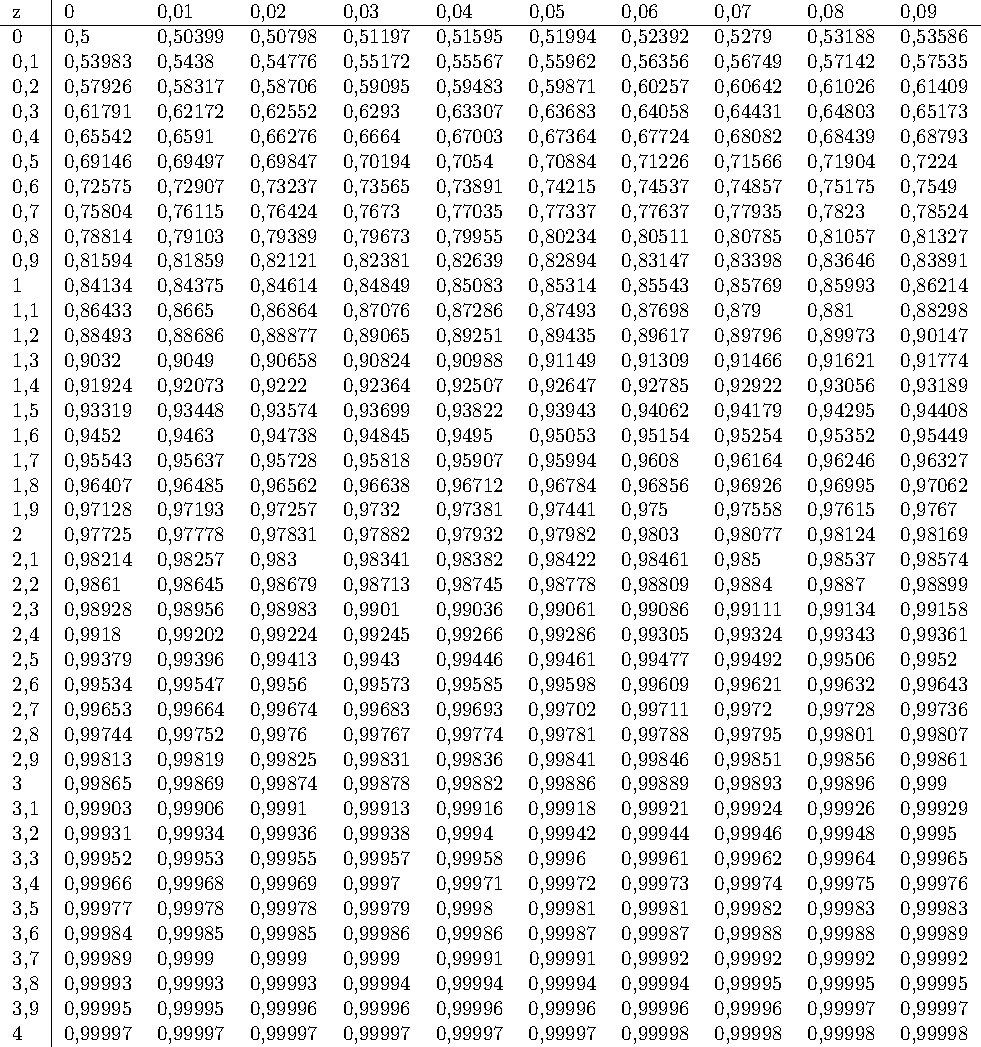
\includegraphics[page=1,width=1\textwidth]{probabilidad/distribucion_normal}
\end{column}
\end{columns}


\end{frame}

\begin{frame}{Cálculo práctico de la probabilidad de la Normal:}
\begin{columns}
\begin{column}{0.6\textwidth}
\begin{block}{}
... y que refleja:

$$P\left(Z\leq k \right), \ \  k \in \left[ 0 , 4'09 \right]$$
\begin{center}
    %\documentclass{article}
%\usepackage{pgfplots}
%\usetikzlibrary{math}
%\begin{document}



\begin{tikzpicture}[scale=0.7]

\pgfmathdeclarefunction{gauss}{2}{%
  \pgfmathparse{1/(#2*sqrt(2*pi))*exp(-((x-#1)^2)/(2*#2^2))}%
}

\tikzmath{
			\conf = 0; \crit= 1.05; \a=round(1-\conf)/2,2);
          }

%\begin{axis}[
%  no markers, domain=0:10, samples=100,
%  axis lines*=left, xlabel=$x$, ylabel=$y$,
%  every axis y label/.style={at=(current axis.above origin),anchor=south},
%  every axis x label/.style={at=(current axis.right of origin),anchor=west},
%  height=5cm, width=12cm,
%  xtick={4,6.5}, ytick=\empty,
%  enlargelimits=false, clip=false, axis on top,
%  grid = major
%  ]
%  \addplot [fill=cyan!20, draw=none, domain=0:5.96] {gauss(6.5,1)} \closedcycle;
%  \addplot [very thick,cyan!50!black] {gauss(4,1)};
%  \addplot [very thick,cyan!50!black] {gauss(6.5,1)};
%
%
%%\draw [yshift=-0.6cm, latex-latex](axis cs:4,0) -- node [fill=white] {$1.96\sigma$} (axis cs:5.96,0);
%\end{axis}

\begin{axis}[
  no markers, domain=-5:5, samples=100,
  axis lines=left, 
  %xlabel=$xa$, ylabel=$ya$,
  %every axis y label/.style={at=(current axis.above origin),anchor=south},
  %every axis x label/.style={at=(current axis.right of origin),anchor=west},
  height=5cm, width=12cm,
  xtick={\crit}, ytick=\empty,
  xticklabels = { $k$},
  enlargelimits=false, clip=false, axis on top,
  %grid = major
  ]
  \addplot [fill=cyan!20, draw=none, domain=-5:\crit] {gauss(0,1)} \closedcycle;
  \addplot [very thick,cyan!50!black] {gauss(0,1)};
  %\addplot [very thick,cyan!50!black] {gauss(6.5,1)};
  


%\draw [yshift=-0.6cm, latex-latex](axis cs:4,0) -- node [fill=white] {$1.96\sigma$} (axis cs:5.96,0);
\end{axis}
\node[] at (5,1.5) {$P\left(Z \leq k \right) $};	




\end{tikzpicture}

%\end{document}
\end{center}
\end{block}
\end{column}
\begin{column}{0.4\textwidth}
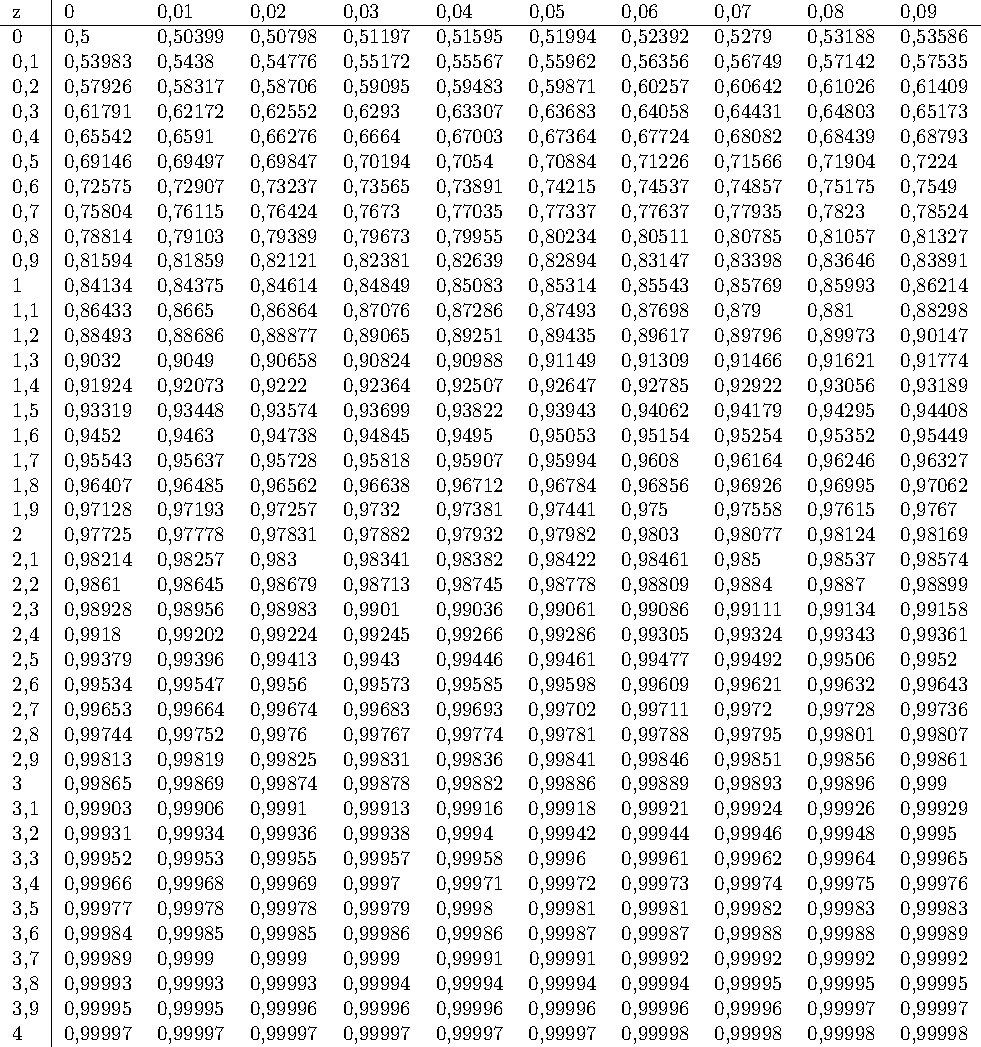
\includegraphics[page=1,width=1\textwidth]{probabilidad/distribucion_normal}
\end{column}
\end{columns}


\end{frame}

\begin{frame}{Cálculo en la $Z \sim \mathcal{N}(0,\,1)$ o normal estándar}
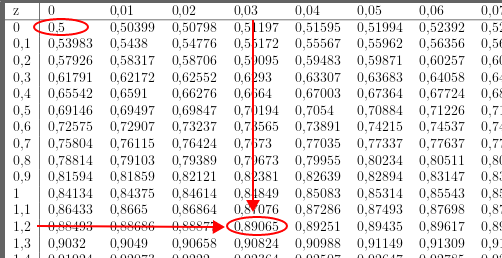
\includegraphics[page=1,width=0.8\textwidth]{probabilidad/calculonormal.png}
\begin{itemize} [<+->]
    \item $P\left(Z\leq 0 \right)=0.5 $. Ya que en este caso $k=0=0.00$ la suma del valor de la fila 0 con el valor de la columna 0 me da el valor de $k$, y la probabilidad asociada es $0.5$
    \item $P\left(Z\leq 1.23 \right)= 0.89065$. En este caso la probabilidad asociada a 1.23 se busca en la fila 1.2 y la columna 0.03 
\end{itemize}



\end{frame}

\begin{frame}{Cálculo en la $Z \sim \mathcal{N}(0,\,1)$ o normal estándar} 
\begin{block}{}
    Las probabilidades en conjuntos de valores de la distribución que no se puedan obtener directamente de la tabla se transformarán en operaciones con probabilidades que sí estén en la tabla:
\end{block}
Veamos algunos ejemplos:
\end{frame}


\begin{frame}{Cálculo en la $Z \sim \mathcal{N}(0,\,1)$ o normal estándar}
\begin{block}{Ejemplo}
$P\left(Z\geq 1.23 \right)= 1 - P\left(Z\leq 1.23 \right) = 1 - 0.89065= 0.10935$.
\end{block}
Basta fijarse en la relación que hay entre las áreas:
\begin{center}
   %\documentclass{article}
%\usepackage{pgfplots}
%\usetikzlibrary{math}
%\begin{document}



\begin{tikzpicture}[scale=0.5]

\pgfmathdeclarefunction{gauss}{2}{%
  \pgfmathparse{1/(#2*sqrt(2*pi))*exp(-((x-#1)^2)/(2*#2^2))}%
}

\tikzmath{
			\conf = 0; \crit= 1.05; \a=round(1-\conf)/2,2);
          }

%\begin{axis}[
%  no markers, domain=0:10, samples=100,
%  axis lines*=left, xlabel=$x$, ylabel=$y$,
%  every axis y label/.style={at=(current axis.above origin),anchor=south},
%  every axis x label/.style={at=(current axis.right of origin),anchor=west},
%  height=5cm, width=12cm,
%  xtick={4,6.5}, ytick=\empty,
%  enlargelimits=false, clip=false, axis on top,
%  grid = major
%  ]
%  \addplot [fill=cyan!20, draw=none, domain=0:5.96] {gauss(6.5,1)} \closedcycle;
%  \addplot [very thick,cyan!50!black] {gauss(4,1)};
%  \addplot [very thick,cyan!50!black] {gauss(6.5,1)};
%
%
%%\draw [yshift=-0.6cm, latex-latex](axis cs:4,0) -- node [fill=white] {$1.96\sigma$} (axis cs:5.96,0);
%\end{axis}

\begin{axis}[
  no markers, domain=-5:5, samples=100,
  axis lines=left, 
  %xlabel=$xa$, ylabel=$ya$,
  %every axis y label/.style={at=(current axis.above origin),anchor=south},
  %every axis x label/.style={at=(current axis.right of origin),anchor=west},
  height=5cm, width=12cm,
  xtick={\crit}, ytick=\empty,
  xticklabels = { $k$},
  enlargelimits=false, clip=false, axis on top,
  %grid = major
  ]
  \addplot [fill=cyan!20, draw=none, domain=\crit:5] {gauss(0,1)} \closedcycle;
  \addplot [very thick,cyan!50!black] {gauss(0,1)};
  %\addplot [very thick,cyan!50!black] {gauss(6.5,1)};
  


%\draw [yshift=-0.6cm, latex-latex](axis cs:4,0) -- node [fill=white] {$1.96\sigma$} (axis cs:5.96,0);
\end{axis}
\node[] at (7,0.5) {$P\left(Z \geq k \right) $};	




\end{tikzpicture}

%\end{document} 
\end{center}

\begin{columns}
\begin{column}{0.5\textwidth}
 %\documentclass{article}
%\usepackage{pgfplots}
%\usetikzlibrary{math}
%\begin{document}



\begin{tikzpicture}[scale=0.5]

\pgfmathdeclarefunction{gauss}{2}{%
  \pgfmathparse{1/(#2*sqrt(2*pi))*exp(-((x-#1)^2)/(2*#2^2))}%
}

\tikzmath{
			\conf = 0; \crit= 1.05; \a=round(1-\conf)/2,2);
          }

%\begin{axis}[
%  no markers, domain=0:10, samples=100,
%  axis lines*=left, xlabel=$x$, ylabel=$y$,
%  every axis y label/.style={at=(current axis.above origin),anchor=south},
%  every axis x label/.style={at=(current axis.right of origin),anchor=west},
%  height=5cm, width=12cm,
%  xtick={4,6.5}, ytick=\empty,
%  enlargelimits=false, clip=false, axis on top,
%  grid = major
%  ]
%  \addplot [fill=cyan!20, draw=none, domain=0:5.96] {gauss(6.5,1)} \closedcycle;
%  \addplot [very thick,cyan!50!black] {gauss(4,1)};
%  \addplot [very thick,cyan!50!black] {gauss(6.5,1)};
%
%
%%\draw [yshift=-0.6cm, latex-latex](axis cs:4,0) -- node [fill=white] {$1.96\sigma$} (axis cs:5.96,0);
%\end{axis}

\begin{axis}[
  no markers, domain=-5:5, samples=100,
  axis lines=left, 
  %xlabel=$xa$, ylabel=$ya$,
  %every axis y label/.style={at=(current axis.above origin),anchor=south},
  %every axis x label/.style={at=(current axis.right of origin),anchor=west},
  height=5cm, width=12cm,
  xtick={\crit}, ytick=\empty,
  xticklabels = { $k$},
  enlargelimits=false, clip=false, axis on top,
  %grid = major
  ]
  \addplot [fill=cyan!20, draw=none, domain=-5:5] {gauss(0,1)} \closedcycle;
  \addplot [very thick,cyan!50!black] {gauss(0,1)};
  %\addplot [very thick,cyan!50!black] {gauss(6.5,1)};
  


%\draw [yshift=-0.6cm, latex-latex](axis cs:4,0) -- node [fill=white] {$1.96\sigma$} (axis cs:5.96,0);
\end{axis}
\node[] at (5.25,1.5) {$1$};	




\end{tikzpicture}

%\end{document}
\end{column}
\begin{column}{0.5\textwidth}
 %\documentclass{article}
%\usepackage{pgfplots}
%\usetikzlibrary{math}
%\begin{document}



\begin{tikzpicture}[scale=0.5]

\pgfmathdeclarefunction{gauss}{2}{%
  \pgfmathparse{1/(#2*sqrt(2*pi))*exp(-((x-#1)^2)/(2*#2^2))}%
}

\tikzmath{
			\conf = 0; \crit= 1.05; \a=round(1-\conf)/2,2);
          }

%\begin{axis}[
%  no markers, domain=0:10, samples=100,
%  axis lines*=left, xlabel=$x$, ylabel=$y$,
%  every axis y label/.style={at=(current axis.above origin),anchor=south},
%  every axis x label/.style={at=(current axis.right of origin),anchor=west},
%  height=5cm, width=12cm,
%  xtick={4,6.5}, ytick=\empty,
%  enlargelimits=false, clip=false, axis on top,
%  grid = major
%  ]
%  \addplot [fill=cyan!20, draw=none, domain=0:5.96] {gauss(6.5,1)} \closedcycle;
%  \addplot [very thick,cyan!50!black] {gauss(4,1)};
%  \addplot [very thick,cyan!50!black] {gauss(6.5,1)};
%
%
%%\draw [yshift=-0.6cm, latex-latex](axis cs:4,0) -- node [fill=white] {$1.96\sigma$} (axis cs:5.96,0);
%\end{axis}

\begin{axis}[
  no markers, domain=-5:5, samples=100,
  axis lines=left, 
  %xlabel=$xa$, ylabel=$ya$,
  %every axis y label/.style={at=(current axis.above origin),anchor=south},
  %every axis x label/.style={at=(current axis.right of origin),anchor=west},
  height=5cm, width=12cm,
  xtick={\crit}, ytick=\empty,
  xticklabels = { $k$},
  enlargelimits=false, clip=false, axis on top,
  %grid = major
  ]
  \addplot [fill=cyan!20, draw=none, domain=-5:\crit] {gauss(0,1)} \closedcycle;
  \addplot [very thick,cyan!50!black] {gauss(0,1)};
  %\addplot [very thick,cyan!50!black] {gauss(6.5,1)};
  


%\draw [yshift=-0.6cm, latex-latex](axis cs:4,0) -- node [fill=white] {$1.96\sigma$} (axis cs:5.96,0);
\end{axis}
\node[] at (5,1.5) {$P\left(Z \leq k \right) $};	




\end{tikzpicture}

%\end{document}

\end{column}
\end{columns}
\end{frame}

\begin{frame}{Cálculo en la $Z \sim \mathcal{N}(0,\,1)$ o normal estándar}
\begin{block}{Ejemplo}
$P\left(Z\leq -2.15 \right)=P\left(Z\geq 2.15 \right)=1-P\left(Z\leq 2.15 \right)=1-0.98422=0.01578$.
\end{block}
Basta fijarse en la relación que hay entre las áreas:
\begin{center}
   %\documentclass{article}
%\usepackage{pgfplots}
%\usetikzlibrary{math}
%\begin{document}



\begin{tikzpicture}[scale=0.5]

\pgfmathdeclarefunction{gauss}{2}{%
  \pgfmathparse{1/(#2*sqrt(2*pi))*exp(-((x-#1)^2)/(2*#2^2))}%
}

\tikzmath{
			\conf = 0; \crit= 1.05; \a=round(1-\conf)/2,2);
          }

%\begin{axis}[
%  no markers, domain=0:10, samples=100,
%  axis lines*=left, xlabel=$x$, ylabel=$y$,
%  every axis y label/.style={at=(current axis.above origin),anchor=south},
%  every axis x label/.style={at=(current axis.right of origin),anchor=west},
%  height=5cm, width=12cm,
%  xtick={4,6.5}, ytick=\empty,
%  enlargelimits=false, clip=false, axis on top,
%  grid = major
%  ]
%  \addplot [fill=cyan!20, draw=none, domain=0:5.96] {gauss(6.5,1)} \closedcycle;
%  \addplot [very thick,cyan!50!black] {gauss(4,1)};
%  \addplot [very thick,cyan!50!black] {gauss(6.5,1)};
%
%
%%\draw [yshift=-0.6cm, latex-latex](axis cs:4,0) -- node [fill=white] {$1.96\sigma$} (axis cs:5.96,0);
%\end{axis}

\begin{axis}[
  no markers, domain=-5:5, samples=100,
  axis lines=left, 
  %xlabel=$xa$, ylabel=$ya$,
  %every axis y label/.style={at=(current axis.above origin),anchor=south},
  %every axis x label/.style={at=(current axis.right of origin),anchor=west},
  height=5cm, width=12cm,
  xtick={-\crit, 0,\crit}, ytick=\empty,
  xticklabels = {$-k$,$0$, $k$},
  enlargelimits=false, clip=false, axis on top,
  %grid = major
  ]
  \addplot [fill=cyan!20, draw=none, domain=-5:-\crit] {gauss(0,1)} \closedcycle;
  \addplot [fill=cyan!20, draw=none, domain=\crit:5] {gauss(0,1)} \closedcycle;
  \addplot [very thick,cyan!50!black] {gauss(0,1)};
  %\addplot [very thick,cyan!50!black] {gauss(6.5,1)};
  


%\draw [yshift=-0.6cm, latex-latex](axis cs:4,0) -- node [fill=white] {$1.96\sigma$} (axis cs:5.96,0);
\end{axis}
\node[] at (8,0.5) {$P\left(Z \geq k \right) $};
\node[] at (2.5,0.5) {$P\left(Z \leq -k \right) $};	




\end{tikzpicture}

%\end{document} 
\end{center}
\end{frame}

\begin{frame}{Cálculo en la $Z \sim \mathcal{N}(0,\,1)$ o normal estándar}
\begin{block}{Ejemplo}
$P\left( -1.3 < Z < 3.1\right)=P\left( Z < 3.1\right)-P\left(  Z < -1.3\right)=
    P\left( Z < 3.1\right) - \left[ 1 - P\left(  Z < 1.3\right) \right]= 0.99903 - 1 + 0.9032 = 0.90223$.
\end{block}
Basta fijarse en la relación que hay entre las áreas:
\begin{center}
   %\documentclass{article}
%\usepackage{pgfplots}
%\usetikzlibrary{math}
%\begin{document}



\begin{tikzpicture}[scale=0.5]

\pgfmathdeclarefunction{gauss}{2}{%
  \pgfmathparse{1/(#2*sqrt(2*pi))*exp(-((x-#1)^2)/(2*#2^2))}%
}

\tikzmath{
			\conf = 0.96; \crit= 2.05; \a=round(1-\conf)/2,2);
          }

%\begin{axis}[
%  no markers, domain=0:10, samples=100,
%  axis lines*=left, xlabel=$x$, ylabel=$y$,
%  every axis y label/.style={at=(current axis.above origin),anchor=south},
%  every axis x label/.style={at=(current axis.right of origin),anchor=west},
%  height=5cm, width=12cm,
%  xtick={4,6.5}, ytick=\empty,
%  enlargelimits=false, clip=false, axis on top,
%  grid = major
%  ]
%  \addplot [fill=cyan!20, draw=none, domain=0:5.96] {gauss(6.5,1)} \closedcycle;
%  \addplot [very thick,cyan!50!black] {gauss(4,1)};
%  \addplot [very thick,cyan!50!black] {gauss(6.5,1)};
%
%
%%\draw [yshift=-0.6cm, latex-latex](axis cs:4,0) -- node [fill=white] {$1.96\sigma$} (axis cs:5.96,0);
%\end{axis}

\begin{axis}[
  no markers, domain=-5:5, samples=100,
  axis lines=left, 
  %xlabel=$xa$, ylabel=$ya$,
  %every axis y label/.style={at=(current axis.above origin),anchor=south},
  %every axis x label/.style={at=(current axis.right of origin),anchor=west},
  height=5cm, width=12cm,
  xtick={-1,0,\crit}, ytick=\empty,
  xticklabels = {$a$, $0$, $b$},
  enlargelimits=false, clip=false, axis on top,
  %grid = major
  ]
  \addplot [fill=cyan!20, draw=none, domain=-1:\crit] {gauss(0,1)} \closedcycle;
  \addplot [very thick,cyan!50!black] {gauss(0,1)};
  %\addplot [very thick,cyan!50!black] {gauss(6.5,1)};
  


%\draw [yshift=-0.6cm, latex-latex](axis cs:4,0) -- node [fill=white] {$1.96\sigma$} (axis cs:5.96,0);
\end{axis}
\node[] at (5.5,1.5) {$P\left(a < Z < b \right) $};	




\end{tikzpicture}

%\end{document} 
\end{center}

\begin{columns}
\begin{column}{0.5\textwidth}
 %\documentclass{article}
%\usepackage{pgfplots}
%\usetikzlibrary{math}
%\begin{document}



\begin{tikzpicture}[scale=0.5]

\pgfmathdeclarefunction{gauss}{2}{%
  \pgfmathparse{1/(#2*sqrt(2*pi))*exp(-((x-#1)^2)/(2*#2^2))}%
}

\tikzmath{
			\conf = 0.96; \crit= 2.05; \a=round(1-\conf)/2,2);
          }

%\begin{axis}[
%  no markers, domain=0:10, samples=100,
%  axis lines*=left, xlabel=$x$, ylabel=$y$,
%  every axis y label/.style={at=(current axis.above origin),anchor=south},
%  every axis x label/.style={at=(current axis.right of origin),anchor=west},
%  height=5cm, width=12cm,
%  xtick={4,6.5}, ytick=\empty,
%  enlargelimits=false, clip=false, axis on top,
%  grid = major
%  ]
%  \addplot [fill=cyan!20, draw=none, domain=0:5.96] {gauss(6.5,1)} \closedcycle;
%  \addplot [very thick,cyan!50!black] {gauss(4,1)};
%  \addplot [very thick,cyan!50!black] {gauss(6.5,1)};
%
%
%%\draw [yshift=-0.6cm, latex-latex](axis cs:4,0) -- node [fill=white] {$1.96\sigma$} (axis cs:5.96,0);
%\end{axis}

\begin{axis}[
  no markers, domain=-5:5, samples=100,
  axis lines=left, 
  %xlabel=$xa$, ylabel=$ya$,
  %every axis y label/.style={at=(current axis.above origin),anchor=south},
  %every axis x label/.style={at=(current axis.right of origin),anchor=west},
  height=5cm, width=12cm,
  xtick={-1,0,\crit}, ytick=\empty,
  xticklabels = {$a$, $0$, $b$},
  enlargelimits=false, clip=false, axis on top,
  %grid = major
  ]
  \addplot [fill=cyan!20, draw=none, domain=-5:\crit] {gauss(0,1)} \closedcycle;
  \addplot [very thick,cyan!50!black] {gauss(0,1)};
  %\addplot [very thick,cyan!50!black] {gauss(6.5,1)};
  


%\draw [yshift=-0.6cm, latex-latex](axis cs:4,0) -- node [fill=white] {$1.96\sigma$} (axis cs:5.96,0);
\end{axis}
\node[] at (5.5,1.5) {$P\left(Z < b \right) $};	




\end{tikzpicture}

%\end{document}
\end{column}
\begin{column}{0.5\textwidth}
 %\documentclass{article}
%\usepackage{pgfplots}
%\usetikzlibrary{math}
%\begin{document}



\begin{tikzpicture}[scale=0.5]

\pgfmathdeclarefunction{gauss}{2}{%
  \pgfmathparse{1/(#2*sqrt(2*pi))*exp(-((x-#1)^2)/(2*#2^2))}%
}

\tikzmath{
			\conf = 0.96; \crit= 2.05; \a=round(1-\conf)/2,2);
          }

%\begin{axis}[
%  no markers, domain=0:10, samples=100,
%  axis lines*=left, xlabel=$x$, ylabel=$y$,
%  every axis y label/.style={at=(current axis.above origin),anchor=south},
%  every axis x label/.style={at=(current axis.right of origin),anchor=west},
%  height=5cm, width=12cm,
%  xtick={4,6.5}, ytick=\empty,
%  enlargelimits=false, clip=false, axis on top,
%  grid = major
%  ]
%  \addplot [fill=cyan!20, draw=none, domain=0:5.96] {gauss(6.5,1)} \closedcycle;
%  \addplot [very thick,cyan!50!black] {gauss(4,1)};
%  \addplot [very thick,cyan!50!black] {gauss(6.5,1)};
%
%
%%\draw [yshift=-0.6cm, latex-latex](axis cs:4,0) -- node [fill=white] {$1.96\sigma$} (axis cs:5.96,0);
%\end{axis}

\begin{axis}[
  no markers, domain=-5:5, samples=100,
  axis lines=left, 
  %xlabel=$xa$, ylabel=$ya$,
  %every axis y label/.style={at=(current axis.above origin),anchor=south},
  %every axis x label/.style={at=(current axis.right of origin),anchor=west},
  height=5cm, width=12cm,
  xtick={-1,0,\crit}, ytick=\empty,
  xticklabels = {$a$, $0$, $b$},
  enlargelimits=false, clip=false, axis on top,
  %grid = major
  ]
  \addplot [fill=cyan!20, draw=none, domain=-5:-1] {gauss(0,1)} \closedcycle;
  \addplot [very thick,cyan!50!black] {gauss(0,1)};
  %\addplot [very thick,cyan!50!black] {gauss(6.5,1)};
  


%\draw [yshift=-0.6cm, latex-latex](axis cs:4,0) -- node [fill=white] {$1.96\sigma$} (axis cs:5.96,0);
\end{axis}
\node[] at (3,1.5) {$P\left(Z < a \right) $};	




\end{tikzpicture}

%\end{document}
\end{column}
\end{columns}
\end{frame}

\begin{frame}{Cálculo en la $Z \sim \mathcal{N}(0,\,1)$ o normal estándar}
\begin{block}{Cálculo del valor de la variable a partir de la probabilidad}
El uso de la tabla normal nos permite realizar el proceso inverso. Es decir, fijada una probabilidad $Pr$, encontrar el valor de la variable $k$ que cumpla:
$$P(Z<=k)=Pr$$
    \begin{center}
        %\documentclass{article}
%\usepackage{pgfplots}
%\usetikzlibrary{math}
%\begin{document}



\begin{tikzpicture}[scale=0.7]

\pgfmathdeclarefunction{gauss}{2}{%
  \pgfmathparse{1/(#2*sqrt(2*pi))*exp(-((x-#1)^2)/(2*#2^2))}%
}

\tikzmath{
			\conf = 0; \crit= 1.05; \a=round(1-\conf)/2,2);
          }

%\begin{axis}[
%  no markers, domain=0:10, samples=100,
%  axis lines*=left, xlabel=$x$, ylabel=$y$,
%  every axis y label/.style={at=(current axis.above origin),anchor=south},
%  every axis x label/.style={at=(current axis.right of origin),anchor=west},
%  height=5cm, width=12cm,
%  xtick={4,6.5}, ytick=\empty,
%  enlargelimits=false, clip=false, axis on top,
%  grid = major
%  ]
%  \addplot [fill=cyan!20, draw=none, domain=0:5.96] {gauss(6.5,1)} \closedcycle;
%  \addplot [very thick,cyan!50!black] {gauss(4,1)};
%  \addplot [very thick,cyan!50!black] {gauss(6.5,1)};
%
%
%%\draw [yshift=-0.6cm, latex-latex](axis cs:4,0) -- node [fill=white] {$1.96\sigma$} (axis cs:5.96,0);
%\end{axis}

\begin{axis}[
  no markers, domain=-5:5, samples=100,
  axis lines=left, 
  %xlabel=$xa$, ylabel=$ya$,
  %every axis y label/.style={at=(current axis.above origin),anchor=south},
  %every axis x label/.style={at=(current axis.right of origin),anchor=west},
  height=5cm, width=12cm,
  xtick={\crit}, ytick=\empty,
  xticklabels = { $k$},
  enlargelimits=false, clip=false, axis on top,
  %grid = major
  ]
  \addplot [fill=cyan!20, draw=none, domain=-5:\crit] {gauss(0,1)} \closedcycle;
  \addplot [very thick,cyan!50!black] {gauss(0,1)};
  %\addplot [very thick,cyan!50!black] {gauss(6.5,1)};
  


%\draw [yshift=-0.6cm, latex-latex](axis cs:4,0) -- node [fill=white] {$1.96\sigma$} (axis cs:5.96,0);
\end{axis}
\node[] at (5,1.5) {$Pr$};	




\end{tikzpicture}

%\end{document}

    \end{center}
\end{block}

\end{frame}

\begin{frame}{Ejemplo}

Dada $Z \sim \mathcal{N}(0,\,1)$, calcula el valor de la variable sabiendo que la probabilidad de que tome un valor menor que ese es de un 85\%. 

$$P(Z<=k)=0.85$$
    \begin{center}
        %\documentclass{article}
%\usepackage{pgfplots}
%\usetikzlibrary{math}
%\begin{document}



\begin{tikzpicture}[scale=0.5]

\pgfmathdeclarefunction{gauss}{2}{%
  \pgfmathparse{1/(#2*sqrt(2*pi))*exp(-((x-#1)^2)/(2*#2^2))}%
}

\tikzmath{
			\conf = 0; \crit= 1.05; \a=round(1-\conf)/2,2);
          }

%\begin{axis}[
%  no markers, domain=0:10, samples=100,
%  axis lines*=left, xlabel=$x$, ylabel=$y$,
%  every axis y label/.style={at=(current axis.above origin),anchor=south},
%  every axis x label/.style={at=(current axis.right of origin),anchor=west},
%  height=5cm, width=12cm,
%  xtick={4,6.5}, ytick=\empty,
%  enlargelimits=false, clip=false, axis on top,
%  grid = major
%  ]
%  \addplot [fill=cyan!20, draw=none, domain=0:5.96] {gauss(6.5,1)} \closedcycle;
%  \addplot [very thick,cyan!50!black] {gauss(4,1)};
%  \addplot [very thick,cyan!50!black] {gauss(6.5,1)};
%
%
%%\draw [yshift=-0.6cm, latex-latex](axis cs:4,0) -- node [fill=white] {$1.96\sigma$} (axis cs:5.96,0);
%\end{axis}

\begin{axis}[
  no markers, domain=-5:5, samples=100,
  axis lines=left, 
  %xlabel=$xa$, ylabel=$ya$,
  %every axis y label/.style={at=(current axis.above origin),anchor=south},
  %every axis x label/.style={at=(current axis.right of origin),anchor=west},
  height=5cm, width=12cm,
  xtick={\crit}, ytick=\empty,
  xticklabels = { $k$},
  enlargelimits=false, clip=false, axis on top,
  %grid = major
  ]
  \addplot [fill=cyan!20, draw=none, domain=-5:\crit] {gauss(0,1)} \closedcycle;
  \addplot [very thick,cyan!50!black] {gauss(0,1)};
  %\addplot [very thick,cyan!50!black] {gauss(6.5,1)};
  


%\draw [yshift=-0.6cm, latex-latex](axis cs:4,0) -- node [fill=white] {$1.96\sigma$} (axis cs:5.96,0);
\end{axis}
\node[] at (5,1.5) {$0.75$};	




\end{tikzpicture}

%\end{document}
    \end{center}

Vamos a la tabla y buscamos los dos valores seguidos de la tabla entre los que se quede el $0.85$ y encontramos:
$$0.84849 < 0.85 < 0.85083 $$
Como queda más cerca del $0.85083$, me quedo con la celda correspondiente a la fila $1$ y columna $0.04$  $\Rightarrow k=1.04$.
\end{frame}

\begin{frame}{Cálculo en $X \sim \mathcal{N}(\mu,\,\sigma)$ - Tipificación}
Para manejar $X \sim \mathcal{N}(\mu,\,\sigma)$ reduciremos los cálculos a cálculos en la $Z \sim \mathcal{N}(0,\,1)$ a partir de la siguiente propiedad:

\begin{block}{}
$$ Si \  X \sim \mathcal{N}(\mu,\,\sigma) \Rightarrow X^{'}=\frac{X - \mu}{\sigma} \sim \mathcal{N}(0,\,1) $$
\end{block}

\pause

Al proceso de transformar la variable anterior a una $Z\sim \mathcal{N}(0,\,1)$ se denomina \textbf{tipificarla}.


\end{frame}



\begin{frame}{Ejemplos}

\begin{itemize}[<+->]
    \item $X \sim \mathcal{N}(1,\,2) \to P(X<=2.32)=P(X'<=\frac{2.32-1}{2})=P(Z<=0.66)=0.74537$
    \item $X \sim \mathcal{N}(5,\,3) \to P(X<=3.59)=P(X'<=\frac{3.59-5}{3})=P(Z<=-0.47)=1-P(Z<=0.47)=1-0.68082=0.31918$
\end{itemize}
\end{frame}


\begin{frame}{Estimación Puntual de la media y la varianza}
Dada una población de media $\mu$ y desviación típica $\sigma$
\begin{block}{Estimación de la media}
 Un buen estimador de $\mu$ es la \textbf{media muestral} $\overline{x}$:
$$\overline{x}= \frac{x_1 + x_2 + ....+x_n} {n}=\frac{{\sum_{i=1}^n x_i }}{n}$$
\end{block}
\pause
\begin{block}{Estimación de la varianza}
Un buen estimador de $\sigma^2$ es la cuasivarianza muestral:
$$\widehat{\sigma}^2=\frac{n-1}{n}s^2$$
siendo $s^2$ la varianza muestral:
$$s^2=\frac{\sum_{i=1}^n x_i^2 }{n} - \bar x^2$$
\end{block}
\end{frame}

\begin{frame}{Ejemplo}
\begin{block}{}
Una muestra aleatoria de 36 personas, empleadas en una gran industria, da el número medio de días al año que faltan al trabajo es $\overline{x} = 12$ con $s^2 = 4$
\end{block}

\begin{itemize}[<+->]
    \item Dar una estimación puntual de $\mu$ (media poblacional)
    \pause 
    \\ Un estimador es la media muestral que en este caso vale 12
    \item Dar una estimación puntual de $\sigma^2$ (varianza poblacional)
    \pause 
    \\ Un estimador es la cuasivarianza muestral:
    $$\widehat{\sigma}^2=\frac{n-1}{n}s^2=\frac{35}{36}\cdot 4\approx 3.9$$
\end{itemize}

\end{frame}


\begin{frame}{Estimación por intervalos}
\begin{block}{}
La estimación puntual sirve de poco mientras
desconozcamos cuál es el grado de aproximación del estimador al parámetro real. Por ese motivo se procede
a la \textbf{estimación mediante un intervalo de confianza}.
\end{block}
\pause
Veremos cómo calcular intervalos de confianza para estimar
\begin{itemize}
    \item La media de la población
    \item La proporción de la población que cumple una característica
\end{itemize}
\end{frame}




\begin{frame}{Distribuciones muestrales}
\begin{block}{} A partir de los diferentes valores que puede tomar una muestra se pude construir una variable aleatoria a la que podemos asociar una probabilidad. Esto nos da una distribución a la que llamaremos \textbf{distribución muestral}

\end{block}    
\pause
\begin{itemize}[<+->]
    \item{Media} La distribución de medias muestrales nos permitirá obtener intervalos de confianza de la media poblacional
    \begin{block}{}
        $$\overline{X} \approx N\left(\mu,\frac{\sigma}{\sqrt{n}}\right)$$
    \end{block}

    \item{Proporción} La distribución de proporciones muestrales nos permitirá obtener intervalos de confianza de la media poblacional
    \begin{block}{}
    $$\widehat{p} \rightarrow N \left ( p , \sqrt{ \frac{p \cdot (1-p)} {n}}\right )$$
    \end{block}
    
\end{itemize}

\end{frame}

\begin{frame}{Ejemplo}


\begin{itemize}[<+->]
    \item  Se ha seleccionado una muestra al azar de 50 mujeres de una población de mayores
de 18 años. En la muestra se ha observado que la media de las 50 tallas es 1,60 m. Si se sabe que
la desviación típica en la población es de 3,3 cm, determina la probabilidad de que la
media de la población no difiere en más de 1 cm de la de la muestra. 
    \item Como $\overline{X} \approx N\left(\mu,\frac{\sigma}{\sqrt{n}}\right)$, tipificando $\frac{\overline{X} -\mu}{\frac{\sigma}{\sqrt{n}}} \rightarrow Z(0,1)$ y por tanto: $P(\mu-1 < \overline{X} < \mu +1)=P(\frac{-1}{\frac{\sigma}{\sqrt{n}}} < Z < \frac{1}{\frac{\sigma}{\sqrt{n}}})\approx 0.967866646858422$
    
\end{itemize}


\end{frame}





\begin{frame}
{Estimación de la media por intervalo de confianza}
A partir de una muestra de tamaño n y un grado de confianza $1-\alpha$: 
\begin{block}{Intervalo de confianza para la media}
$$ \left( \overline{x} - z_{\alpha / 2}\cdot \frac{\sigma}{\sqrt{n}} ,  \overline{x} + z_{\alpha / 2}\cdot \frac{\sigma}{\sqrt{n}}
\right)$$
siendo: \begin{itemize}
\item $\overline{x}$: La media de los datos de la muestra
\item $z_{\alpha / 2}$ o valor crítico: El valor de la distribución normal  $Z\leadsto N\left((0,1\right)$ tal que $P(Z>z_{\alpha / 2})=\frac{\alpha}{2}$ ($\alpha$ es el nivel de significación)
\item $\sigma$: La desviación típica de la distribución de la población (o si no se conoce de un estimador sesgado de la misma)
\item $n$: El tamaño de la muestra
\end{itemize}
\end{block}
\pause

\end{frame}

\begin{frame}
{Ejemplo}
\begin{block}{Problema} La duración de las bombillas de un fabricante es una variable aleatoria con distribución
normal de desviación típica 75 horas. Decidimos tomar un tamaño de la muestra igual a 150, comprobamos la duración de cada
bombilla y calculamos su promedio, que resulta ser 1053 horas. Calcular el intervalo de confianza al 98\%
para la media de la duración de las bombillas del fabricante.
\end{block}
\end{frame}

\begin{frame}{Ejemplo: Solución}
\begin{columns}
\begin{column}{0.5\textwidth}
    \textbf{Datos:} $\overline{x}=1053$, Confianza=$98$\%, $\sigma=75$ y n=150 \\
    $\alpha=1-0.98=0.02 \to \frac{\alpha}{2}=\frac{0.02}{2}=0.01$
    . \\ Por tanto, el valor crítico será: \\
    $P\left(Z \leqslant z_{\alpha / 2} \right)= 0.98 + 0.01 = 0.99 \to z_{\alpha / 2} = 2.33$ \\
    A partir de la definición de intervalo de confianza de la media:
    $$ \left( \overline{x} - z_{\alpha / 2}\cdot \frac{\sigma}{\sqrt{n}} ,  \overline{x} + z_{\alpha / 2}\cdot \frac{\sigma}{\sqrt{n}}
    \right)$$

\end{column}
\begin{column}{0.5\textwidth}
    %\documentclass{article}
%\usepackage{pgfplots}
%\usetikzlibrary{math}
%\begin{document}



\begin{tikzpicture}[scale=0.7]

\pgfmathdeclarefunction{gauss}{2}{%
  \pgfmathparse{1/(#2*sqrt(2*pi))*exp(-((x-#1)^2)/(2*#2^2))}%
}

\tikzmath{
			\conf = 0.98; \crit= 2.33; \a=round(1-\conf)/2,2);
          }

%\begin{axis}[
%  no markers, domain=0:10, samples=100,
%  axis lines*=left, xlabel=$x$, ylabel=$y$,
%  every axis y label/.style={at=(current axis.above origin),anchor=south},
%  every axis x label/.style={at=(current axis.right of origin),anchor=west},
%  height=5cm, width=12cm,
%  xtick={4,6.5}, ytick=\empty,
%  enlargelimits=false, clip=false, axis on top,
%  grid = major
%  ]
%  \addplot [fill=cyan!20, draw=none, domain=0:5.96] {gauss(6.5,1)} \closedcycle;
%  \addplot [very thick,cyan!50!black] {gauss(4,1)};
%  \addplot [very thick,cyan!50!black] {gauss(6.5,1)};
%
%
%%\draw [yshift=-0.6cm, latex-latex](axis cs:4,0) -- node [fill=white] {$1.96\sigma$} (axis cs:5.96,0);
%\end{axis}

\begin{axis}[
  no markers, domain=-5:5, samples=100,
  axis lines=left, 
  %xlabel=$xa$, ylabel=$ya$,
  %every axis y label/.style={at=(current axis.above origin),anchor=south},
  %every axis x label/.style={at=(current axis.right of origin),anchor=west},
  height=5cm, width=12cm,
  xtick={0,\crit}, ytick=\empty,
  xticklabels = {$0$, $z_{\frac{\alpha}{2}}=\crit$},
  enlargelimits=false, clip=false, axis on top,
  %grid = major
  ]
  \addplot [fill=cyan!20, draw=none, domain=-\crit:\crit] {gauss(0,1)} \closedcycle;
  \addplot [very thick,cyan!50!black] {gauss(0,1)};
  %\addplot [very thick,cyan!50!black] {gauss(6.5,1)};
  


%\draw [yshift=-0.6cm, latex-latex](axis cs:4,0) -- node [fill=white] {$1.96\sigma$} (axis cs:5.96,0);
\end{axis}
\node[] at (5.2,1.5) {$\conf$};	
\draw[->]   (\crit+6.5,1)node[right]{$\a$}  --  (\crit+5.6,0.1) ;



\end{tikzpicture}

%\end{document}
\end{column}
\end{columns}
    
    Operando nos queda:
    $$ \left( 1053 - 2.33 \cdot \frac{75}{\sqrt{150}} ,  1053 + 2.33 \cdot \frac{75}{\sqrt{150}}
    \right)=\left(1038.73 ,  1067.27\right)
    $$
\end{frame}


\begin{frame}{Error máximo del intervalo de la media}
\begin{center}
        \begin{tikzpicture}[scale=0.4]
        
        \tikzmath{
        			\a = -10; \b = 10; \aa = \a -1; \bb = \b + 1 ;
        			\dist = \b - \a; \med = (\a + \b)/2;
                  }
        
        \draw[very thick] (\a,0) -- (\b,0);
        \path [draw=black, fill=white] (\b,0) circle (2pt);
        \path [draw=black, fill=white] (\a,0.0) circle (2pt);
        \draw[latex-latex] (\a - 1.5,0) -- (\b + 1.5,0) ;
        
        % \foreach \x in  {\a,...,\b}
        % \draw[shift={(\x,0)},color=black] (0pt,3pt) -- (0pt,-3pt);
        % \foreach \x in  {\aa,...,\bb}
        % \draw[shift={(\x,0)},color=black] (0pt,0pt) -- (0pt,-3pt) node[below] % {$\pgfmathprintnumber{\x}$};
        \draw[shift={(\a,0)},color=black] (0pt,3pt) -- (0pt,-3pt);
        \draw[shift={(\a,0)},color=black] (0pt,0pt) -- (0pt,-3pt) node[below] {$\overline{x} - z_{\alpha / 2}\cdot \frac{\sigma}{\sqrt{n}}$};
        \draw[shift={(\med,0)},color=black] (0pt,3pt) -- (0pt,-3pt);
        \draw[shift={(\med,0)},color=black] (0pt,0pt) -- (0pt,-3pt) node[below] {$\overline{x}$};
        \draw[shift={(\b,0)},color=black] (0pt,3pt) -- (0pt,-3pt);
        \draw[shift={(\b,0)},color=black] (0pt,0pt) -- (0pt,-3pt) node[below] {$\overline{x} + z_{\alpha / 2}\cdot \frac{\sigma}{\sqrt{n}}$};
        
          \draw[decorate,decoration={brace}, thick]
            (\med,0.2)--(\b,0.2) node[above, midway] 
        {$E=z_{\alpha / 2}\cdot \frac{\sigma}{\sqrt{n}}$}; 
        \end{tikzpicture}
\end{center}

\begin{block}{} $$E=z_{\alpha / 2}\cdot \frac{\sigma}{\sqrt{n}}$$
Es el radio del entorno dado por el intervalo de confianza.
\end{block}

\textbf{NOTA:} Disminuye al aumentar el tamaño de la muestra y por tanto si se quiere garantizar un error determinado para un nivel de confianza habrá que tomar muestras de al menos un \textbf{tamaño determinado de la muestra}:.

\begin{block}{} $$E=z_{\alpha / 2}\cdot \frac{\sigma}{\sqrt{n}} \Rightarrow n =\frac{\sigma^2 \cdot z_{\alpha / 2}^2}{E^2}$$

\end{block}


\end{frame}

\begin{frame}{Ejemplo}


\begin{block}{}
Se desea realizar una investigación para estimar el peso medio de los recién nacidos de madres fumadoras. Se admite un error máximo de 50 gramos, con una confianza del 95\%. Si por estudios anteriores se sabe que la desviación típica del peso medio de tales recién nacidos es de 400 gramos, ¿qué tamaño mínimo de muestra se necesita en la investigación?
\end{block}
    
\end{frame}{}


\begin{frame}{Ejemplo: Solución}

    \textbf{Datos:} $E=50$, Confianza=$95$ y $\sigma=400$ \\
$\alpha=1-0.95=0.05 \to \frac{\alpha}{2}=\frac{0.05}{2}=0.025$
. \\ Por tanto, el valor crítico será: \\
$P\left(Z \leqslant z_{\alpha / 2} \right)= 0.95 + 0.025 = 0.975 \to z_{\alpha / 2} = 1.96$\\ A partir de la definición de error máximo admitido:
$$E=z_{\alpha / 2}\cdot \frac{\sigma}{\sqrt{n}} \to 
n = \left( \frac{z_{\alpha / 2} \cdot \sigma}{E} \right) ^ 2$$
Luego: \\
$$n = \left( \frac{1.96 \cdot 400}{50} \right) ^ 2\approx 245.8534 \to n=246
$$
\end{frame}

\begin{frame}
{Estimación de la proporción por intervalo de confianza}
A partir de una muestra de tamaño n y un grado de confianza $1-\alpha$: 
\begin{block}{Intervalo de confianza para la proporción}
$$ \left( \widehat{p} - z_{\alpha / 2}\cdot \sqrt{\frac{\widehat{p}\cdot\left(1-\overline{p} \right)}{n}} ,  \widehat{p} + z_{\alpha / 2}\cdot \sqrt{\frac{\widehat{p}\cdot\left(1-\widehat{p} \right)}{n}}\right)$$
siendo: \begin{itemize}
\item $\widehat{p}$: La proporción muestral
\item $z_{\alpha / 2}$ o valor crítico:  $P(Z>z_{\alpha / 2})=\frac{\alpha}{2}$ 
\item $\sigma$: La desviación típica de la distribución de la población \item $n$: El tamaño de la muestra
\end{itemize}
\end{block}
Llamaremos error máximo a:
\begin{block}{}
$$E=z_{\alpha / 2}\cdot \sqrt{\frac{\widehat{p}\cdot\left(1-\widehat{p} \right)}{n}}$$
\end{block}

\end{frame}

\begin{frame}
{Ejemplo}
\begin{block}{Problema} Para estimar la proporción de personas con sobrepeso en una población se ha tomado una
muestra aleatoria simple de tamaño 100 personas, de las cuales 21 tienen sobrepeso. Calcular el intervalo
de confianza al 96\% para la proporción de personas con sobrepeso en la población.
\end{block}
\end{frame}

\begin{frame}{Ejemplo: Solución}
\begin{columns}
\begin{column}{0.55\textwidth}
    \textbf{Datos:} $\widehat{p}=0.21$, Confianza=$96$ \\
$\alpha=1-0.96=0.04 \to \frac{\alpha}{2}=\frac{0.04}{2}=0.02$
. \\ Por tanto, el valor crítico será: \\

$P\left(Z \leqslant z_{\alpha / 2} \right)= 0.96 + 0.02 = 0.98 \to z_{\alpha / 2} \approx 2.05$ \\ 
A partir de la definición de error máximo admitido:
$$E=z_{\alpha / 2}\cdot \sqrt{\frac{\widehat{p}\cdot\left(1-\widehat{p} \right)}{n}}\approx 2.05 \cdot \sqrt{\frac{0.21\cdot 0.79}{100}}\approx 0.08$$

\end{column}
\begin{column}{0.45\textwidth}
    %\documentclass{article}
%\usepackage{pgfplots}
%\usetikzlibrary{math}
%\begin{document}



\begin{tikzpicture}[scale=0.45]

\pgfmathdeclarefunction{gauss}{2}{%
  \pgfmathparse{1/(#2*sqrt(2*pi))*exp(-((x-#1)^2)/(2*#2^2))}%
}

\tikzmath{
			\conf = 0.96; \crit= 2.05; \a=round((1-\conf)/2),2);
          }

%\begin{axis}[
%  no markers, domain=0:10, samples=100,
%  axis lines*=left, xlabel=$x$, ylabel=$y$,
%  every axis y label/.style={at=(current axis.above origin),anchor=south},
%  every axis x label/.style={at=(current axis.right of origin),anchor=west},
%  height=5cm, width=12cm,
%  xtick={4,6.5}, ytick=\empty,
%  enlargelimits=false, clip=false, axis on top,
%  grid = major
%  ]
%  \addplot [fill=cyan!20, draw=none, domain=0:5.96] {gauss(6.5,1)} \closedcycle;
%  \addplot [very thick,cyan!50!black] {gauss(4,1)};
%  \addplot [very thick,cyan!50!black] {gauss(6.5,1)};
%
%
%%\draw [yshift=-0.6cm, latex-latex](axis cs:4,0) -- node [fill=white] {$1.96\sigma$} (axis cs:5.96,0);
%\end{axis}

\begin{axis}[
  no markers, domain=-5:5, samples=100,
  axis lines=left, 
  %xlabel=$xa$, ylabel=$ya$,
  %every axis y label/.style={at=(current axis.above origin),anchor=south},
  %every axis x label/.style={at=(current axis.right of origin),anchor=west},
  height=5cm, width=12cm,
  xtick={0,\crit}, ytick=\empty,
  xticklabels = {$0$, $z_{\frac{\alpha}{2}}=\crit$},
  enlargelimits=false, clip=false, axis on top,
  %grid = major
  ]
  \addplot [fill=cyan!20, draw=none, domain=-\crit:\crit] {gauss(0,1)} \closedcycle;
  \addplot [very thick,cyan!50!black] {gauss(0,1)};
  %\addplot [very thick,cyan!50!black] {gauss(6.5,1)};
  


%\draw [yshift=-0.6cm, latex-latex](axis cs:4,0) -- node [fill=white] {$1.96\sigma$} (axis cs:5.96,0);
\end{axis}
\node[] at (5.2,1.5) {$\conf$};	
\draw[->]   (\crit+6.5,1)node[right]{$\a$}  --  (\crit+5.6,0.1) ;



\end{tikzpicture}

%\end{document}
\end{column}
\end{columns}
Luego el intervalo es: $$\left( 0.21 - 0.08 , 0.21 + 0,08 \right) = \left(0.13, 0.29 \right)$$ 
\end{frame}





\end{document}